%
% API
% Abschlussarbeit (Bachelor)
%
% Thema: Erstellung einer Browser Extension zur Usability Evaluierung von beliebigen Web-Applikationen über Heatmaps.
% Betreuer 1: Prof. Dr. Targo Pavlista
% Betreuer 2: Siamak Haschemi
%
% @author Christian Bromann <contact@christian-bromann.com>
%

\section{API}

Die \textbf{API} ist der Datenmotor des Frameworks. Sie ist sowohl für die Datenpersistierung als auch für dessen Auslieferung zuständig. Hinter ihr steckt eine NodeJS Applikation, die als dedizierter Service auf einem Server unter einem bestimmten Port laufen muss. Bei einem Test ist sie in ständiger Verbindung mit der Browser Extension, um möglichst viele Daten aufzunehmen. NodeJS eignet sich hierfür sehr gut, da es event-getrieben agiert und dabei nicht blockierend wirkt. Dies bedeutet, dass alle langandauerenden Aktivitäten, wie z.B. Dateizugriffe, Netzwerk Kommunikationen oder Datenbankzugriffe, bei Seite gepackt werden, bis sie beendet sind und das Ergebnis in einer Funktion verarbeitet werden kann \cite{nonblocking}. Dadurch werden Server-Anfragen parallel abgearbeitet und nicht, wie z.B. bei PHP, sequenziell. Dies sorgt für eine stabile Verbindung zwischen Server API und Extension. Zusätzlicher Vorteil einer NodeJS basierten API Architektur ist die Performance. NodeJS basiert auf Googles hochgeschwindigkeits V8 Engine und sorgt damit für eine deutliche höhere Reaktionszeit beim Server im Vergleich zu Apache-Servern \cite{nodevsphp}.


\subsection{Architektur}

NodeJS bietet in seinen Core-Modulen jegliche Funktionalität, die für den Aufbau einer Anwendung notwendig ist. Zusätzlich können Packages eingebunden werden, die weitere Funktionalität für die Erstellung spezieller Anwendungen bringt. Diese sogenannten NPM\footnote{Node Packaged Modules - \url{https://npmjs.org}} Module werden von der NodeJS Community erstellt und maintained. Die API des \textit{thEvaluator} Frameworks nutzt bspw. \textit{express}\footnote{express - web application framework for node \url{http://expressjs.com/}} als Web-Applikations-Framework, um die Rest-Services zu initialisieren und die Socket Schnittstellen einzubinden. Diese werden über das \textit{Sockel.IO}\footnote{Socket.IO - v9 - \url{http://socket.io}} Modul abstrahiert. Zuletzt bietet die \textit{mongoose}\footnote{mongoose - elegant mongodb object modeling for node.js - \url{http://mongoosejs.com/}} Library eine Abstrahierung zur MongoDB Datenbank. Dabei erhalten jegliche C++ - Bindings der MongoDB Architektur eine entsprechende Verknüpfung mit einer JavaScript Funktion, um den Einsatz in NodeJS möglich zu machen.\\
\\
MongoDB ist eine einfach zu skalierende, agile, dokumenten-orientierte Datenbank, geschrieben in C++. Im Bereich der NoSQL Datenbanken ist das Open Source Projekt marktführend und sehr performant. Im Gegensatz zu einer MySQL Datenbank ist diese schemafrei und erfordert dabei keine starren Tabellen mit festgelegten Spalten. Aufgeteilt wird eine MongoDB-Datenbank in verschiedene Collections, die unabhängig voneinander sind und getrennt auf dem Server gespeichert werden \cite{nosql}. Eine Collection entspricht einer Tabelle einer SQL-Datenbank. Sie enthält jegliche Informationen für ein Datenobjekt. Einträge in einer Collection werden als Dokumente bezeichnet und entsprechen einer Zeile einer SQL-Datenbank. Da MongoDB eine schemafreie Ansatz der Datenpersistierung verfolgt, ist die Struktur einer Collection flexibel und kann immer wieder geändert werden.

\begin{center}
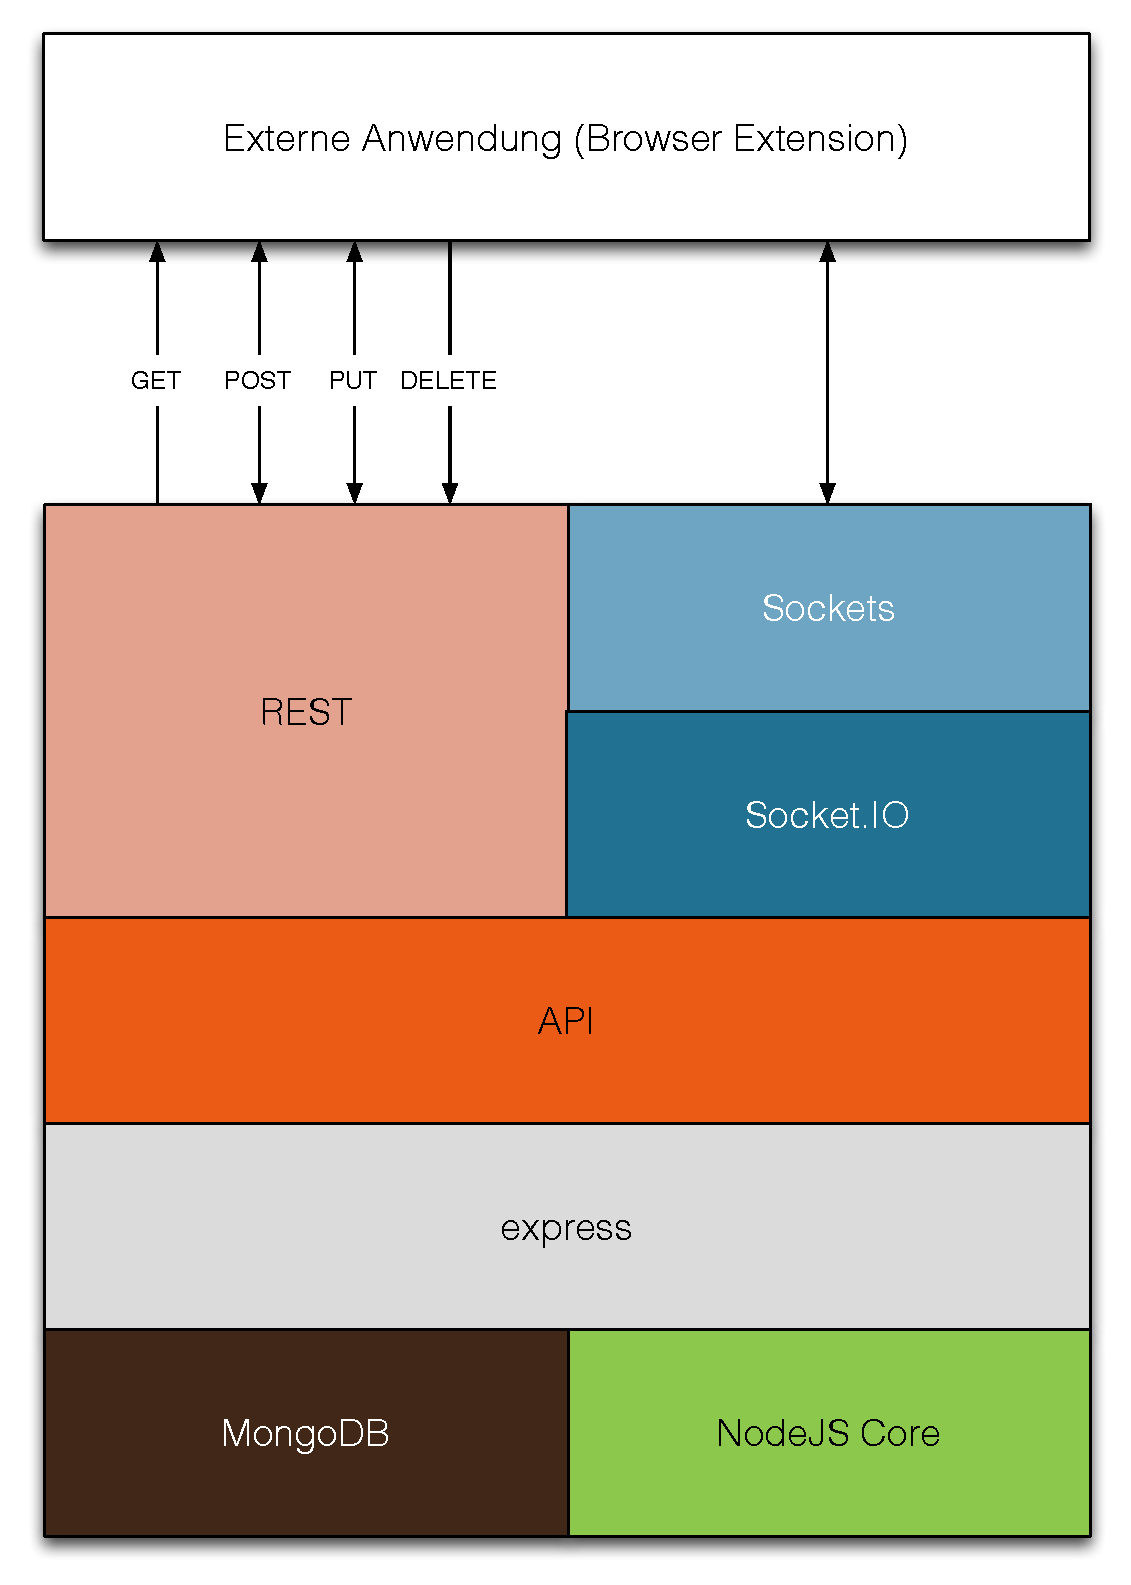
\includegraphics[scale=0.49]{./images/api-architecture}
\end{center}
\begin{figure}[htb]
   \centering
   \caption{Architektur-Schema der API}
    \label{api}
\end{figure}

Der Unterschied zwischen der Rest- und der Socket-Schnittstelle ist, dass beim Letzteren lediglich einmal eine Verbindung zwischen Client und Server hergestellt werden muss. Nach dem Handshake bleibt die TCP Verbindung bestehen und kann Daten in beide Richtungen austauschen. Der HTTP-Overhead, der teilweise mehrere 100 Byte umfassen kann, fällt dadurch weg. Da die API in der Lage sein muss viele Anfragen von der Extension aufzunehmen, spart dies enorm viel Traffic und steigert die Performance.


\subsection{Asynchronität in NodeJS}

Wie zum Anfang des Kapitels beschrieben unterliegt NodeJS einer event-getriebenen und nicht blockierenden Architektur. Es wurde entwickelt von Ryan Dahl und interpretiert Java-Script in der von Google entwickelten V8 Engine. Genauso wie der Browser JavaScript lediglich in einem einzelnen Thread abarbeitet, so tut dies auch NodeJS. Es kommen keine Nebenläufigkeiten vor. Im Gegensatz zu thread-basierten Modellen, bei denen die Threads die meiste Zeit ihres Lebens im blockierten Zustand verbringen, da sie irgendwelche I/O Operationen durchführen oder eine Datenbank-Query abfragen, schiebt NodeJS seine Operationen in einen Event Loop und führt den dazugehörigen Callback erst dann aus, wenn die Operation beendet ist. Gerade bei traffic-lastigen Anwendungen, die ständig erreichbar sein müssen, sind lang blockierende Threads ein Hindernis. Während eine Operation im Event-Loop arbeitet ist NodeJS dagegen in der Lage weiterhin Anfragen anzunehmen und zu verarbeiten. Dadurch ist es perfekt geschaffen zur Erstellung von hoch skalierbaren Echtzeit-Applikationen.\\
\\
Die Methode des event-basierten Verarbeiten von Operationen, zwingt den Entwickler dabei zu einer etwas anderen Denkweise, da Operationsfolgen nicht mehr synchron sondern asynchron abgearbeitet werden müssen. Algorithmen können nicht wie gewohnt untereinander weg geschrieben werden, sondern müssen über Callbacks organisiert werden. Callbacks sind Funktionen, die aufgerufen werden, sobald eine Operation im Event Loop abgearbeitet ist. Sie enthält meist ein Error und ein Ergebnis Objekt der Operation. Listing \ref{async} zeigt ein Beispiel für asynchrone Programmierung.

\vspace{0.6cm}
\begin{lstlisting}[caption=Speichern eines Strings in eine Datei in NodeJS,label=async]
var fs = require('fs');

fs.writeFile('message.txt', 'Hello Node', function (err) {
  if (err) throw err;
  console.log('It\'s saved!');
});

console.log('saved "Hello Node" to message.txt');
\end{lstlisting}

Rein optisch betrachtet, sollte folgende Ausgabe zu erwarten sein:

\begin{verbatim}
It's saved!'
saved "Hello Node" to message.txt
\end{verbatim}

Dies ist aber nicht der Fall! Das Listing zeigt ein Script, welches das \textit{fs} Core Modul\footnote{\textit{fs} steht für File System - \url{http://nodejs.org/api/fs.html}} von NodeJS nutzt, um einen String (\glqq Hello Node\grqq{}) in die Datei \textit{message.txt} zu schreiben. Da Operationen am Dateisystem Zeit beanspruchen (wenn auch nur bruchteilhaft wenig), packt NodeJS diese in den Eventloop und hängt die als Parameter angehängte Callback Funktion an den Listener dieses Events. Dadurch wird die Funktion ausgeführt sobald die Operation beendet ist. Solange NodeJS vom Betriebssystem keine Antwort zum Bearbeitungsstand der Operation erhält, befindet diese sich in einer Art Schlafmodus. NodeJS ist daher in der Lage weiterhin Code auszuführen. Daher wird die zweite \textit{console.log} Ausgabe als erstes angezeigt und erst (bruchteilhaft) kurze Zeit später die Ausgabe aus der Callback Funktion.\\
\\
Bei komplexeren Algorithmen kann es vorkommen, dass mehrere ansynchrone Operationen hintereinander in Abhängigkeit durchgeführt werden müssen. Schnell gerät der Entwickler dabei in die missliche Lage, von zu viel ineinander geschachtelten Funktionen. Listing \ref{nested} zeigt so ein Szenario.

\vspace{0.6cm}
\begin{lstlisting}[caption=\glqq Pyramid of Doom\grqq{} - Undurchsichtiger und unsauberer Code durch zu viele verschachtelte Funktionen,label=nested]
asynchronousFunction(parameter1, function() {
  asynchronousFunction(parameter1, function() {
    asynchronousFunction(parameter1, function() {
      asynchronousFunction(parameter1, function() {
        asynchronousFunction(parameter1, function() {
          console.log('finished!');
        });
      });
    });
  });
});
\end{lstlisting}

Das Beispiel zeigt, dass der Code dadurch ziemlich schnell undurchsichtig und komplex werden kann. Führt man die ansynchronen Funktion in sequenzieller Reihenfolge aus, ist nicht einmal sicher, ob der Callback der letzten asynchronen Funktion auch wirklich als letztes ausgeführt wird.\\
\\
Um den Problemen der Asynchronität und den verschachtelten Probleme aus dem Weg zu gehen, kann man mehrere Wege gehen. Da es eine von Anfang an bestehende Thematik in NodeJS, gibt es viele Entwickler, die sich damit beschäftigt haben. Ein Lösungsansatz wäre die Nutzung von NPM Modulen, die einen Kontrollfluss abbilden, welcher die einer asynchronen nahezu gleich kommt. Einer dieser Module nennt sich \textit{Async.js}\footnote{Erläuterungen zu Async.js sind zu finden auf \url{https://github.com/caolan/async}}. Dieses hilft dem Entwickler über verschiedene Funktionen die Asynchronität zu abstrahieren und den Code mehr synchron aussehen zu lassen. Die Ausführung der Funktion geschieht zwar trotzdem noch asynchron, dennoch sieht die Struktur des Codes deutlich verständlicher aus, wie Listing \ref{asyncjs} zeigt.

\vspace{0.6cm}
\begin{lstlisting}[caption=Sequenzielle Abarbeitung von asynchronen Code durch das Async.js Module,label=asyncjs]
var async = require('async');

async.series([
    asynchronousFunction,
    asynchronousFunction,
    asynchronousFunction,
    // ...
]);
\end{lstlisting}

Das Beispiel zeigt, dass das Modul \textit{Async.js} eine Methode \textit{series} anbietet, welche eine Array mit Funktionen als Parameter aufnimmt und diese sequenziell abarbeitet. Dies ist nur eine Möglichkeit, die das Modul anbietet, um asynchrone Algorithmen so strukturieren. Es bietet für viele Varianten verschiedene Lösungen an.\\
\\
Eine weitere Möglichkeit bietet das Programmierungs-Pradigma der \glqq Promises\grqq{} in Java-Script. Als ein Promise wird ein Objekt bezeichnet, welches eine Funktion \textit{then} verlangt, die zwei Parameter entgegen nimmt \cite{promises}. Dies ist zum Einen ein \textit{success} Callback, welcher aufgerufen wird, wenn die Funktion ohne Fehler ausgeführt wurde, und zum Anderen ein \textit{failure} Callback, welcher ausgeführt wird, wenn die Funktion einen Fehler geworfen hat. Eine asynchrone Funktion liefert laut Paradigma immer ein solches Promise zurück. Die darin enthaltene \textit{then} Funktion tut dies ebenfalls wieder. Dadurch wird es möglich, beliebig viele asynchronen Funktionen miteinander zu verketten. Die Ergebnisse der jeweiligen Funktionen werden dabei immer dem Promise weitergegeben und können somit in der nächsten ansynchronen Funktion weiterverwendet werden. Listing x zeigt die Verwendung von Promises an den bisher orientierten Beispiel vom Anfang des Kapitels. 

\vspace{1.8cm}
\begin{lstlisting}[caption=Sequenzielle Abarbeitung von asynchronen Code durch das Async.js Module,label=asyncjs]
asynchronousFunction().then({
  function(data) {
    // do more asynchronous stuff
    return asynchronousFunction();
  },
  function(err) {
    throw new Error();
  }
}).then({
  function(data) {
    // do more asynchronous stuff
    return asynchronousFunction();
  }
}).then(...);
\end{lstlisting}

Durch die Bereitstellung einer \textit{then} Methode, welches die als Parameter aufgeführten Callbacks erst dann ausführt, sobald die Operation endet, ermöglichen Promises die Vereinfachungen von komplexen Asynchronen Codestrukturen. Da es noch keine offizielle Standardisierung für Promises in JavaScript gibt, wird dieses Feature in dieser Sprache noch nicht unterstützt. Mittlerweile gibt es bereits einen Vorschlag für die Spezifizierung dieses Paradigmas\footnote{CommonJS Promises/A proposal - \url{http://wiki.commonjs.org/wiki/Promises/A}}. Nach Planung von Ecma International, die EcmaScript und somit die Sprache JavaScript standardisieren, wird dieses Feature jedoch erst in EcmaScript 7 aufgenommen. Bis dahin muss sich der Entwickler auf Bibliotheken und Module verlassen, die das Paradigma versuchen abzubilden.\\
\\
Wie die Beispiele zeigen, gibt es Wege, die Asynchronität in den Griff zu bekommen. Für viele Entwickler fällt es im ersten Moment schwer, sich in die asynchrone Verarbeitung hinein zu versetzen und von den Glauben abzukommen, dass alles sequenziell abläuft. Entstehen zu viele verschachtelte Funktionen, da eine Menge asynchroner Operationen ausgeführt werden müssen, so kann es auch sein, dass NodeJS nicht das richtige Werkzeug für die Umsetzung des Vorhabens ist und sich eine thread-basierte Abarbeitung besser eignet. Diese sollte dann der Entwickler von Fall zu Fall unterscheiden.

\subsection{REST Schnittstellen}
% Auflistung mit erforderten Werten / RŸückgabewerten

\subsection{Socket Streams}
% Auflistung mit erforderten Werten / RüŸckgabewerten

\subsection{Persistierung}
% SQL vs NoSQL
% MongoDB / Mongoose